\documentclass[article]{jss}
\usepackage[utf8]{inputenc}

\providecommand{\tightlist}{%
  \setlength{\itemsep}{0pt}\setlength{\parskip}{0pt}}

\author{
Sahir Bhatnagar *\\McGill Univeristy \And Maxime Turgeon *\\McGill University \And James Hanley\\McGill Univeristy \And Olli Saarela\\University of Toronto
}
\title{\pkg{casebase}: An Alternative Framework For Survival Analysis}

\Plainauthor{Sahir Bhatnagar *, Maxime Turgeon *, James Hanley, Olli Saarela}
\Plaintitle{casebase: An Alternative Framework For Survival Analysis}
\Shorttitle{\pkg{casebase}: An Alternative Framework For Survival Analysis}

\Abstract{
The abstract of the article. * joint co-authors
}

\Keywords{keywords, not capitalized, \proglang{Java}}
\Plainkeywords{keywords, not capitalized, Java}

%% publication information
%% \Volume{50}
%% \Issue{9}
%% \Month{June}
%% \Year{2012}
%% \Submitdate{}
%% \Acceptdate{2012-06-04}

\Address{
    Sahir Bhatnagar *\\
  McGill Univeristy\\
  1020 Pine Avenue West Montreal, QC, Canada H3A 1A2\\
  E-mail: \email{sahir.bhatnagar@mail.mcgill.ca}\\
  URL: \url{http://sahirbhatnagar.com/}\\~\\
      Maxime Turgeon *\\
  McGill University\\
  1020 Pine Avenue West Montreal, QC, Canada H3A 1A2\\
  E-mail: \email{maxime.turgeon@mail.mcgill.ca}\\
  URL: \url{http://maxturgeon.ca/}\\~\\
      James Hanley\\
  McGill Univeristy\\
  1020 Pine Avenue West Montreal, QC, Canada H3A 1A2\\
  E-mail: \email{james.hanley@mcgill.ca}\\
  URL: \url{http://www.medicine.mcgill.ca/epidemiology/hanley/}\\~\\
      Olli Saarela\\
  University of Toronto\\
  Dalla Lana School of Public Health, 155 College Street, 6th floor,
  Toronto, Ontario M5T 3M7, Canada\\
  E-mail: \email{olli.saarela@utoronto.ca}\\
  URL: \url{http://individual.utoronto.ca/osaarela/}\\~\\
  }

% Pandoc header

\usepackage{amsmath}

\begin{document}

\section{Code formatting}\label{code-formatting}

Don't use markdown, instead use the more precise latex commands:

\begin{itemize}
\tightlist
\item
  \proglang{Java}
\item
  \pkg{plyr}
\item
  \code{print("abc")}
\end{itemize}

\section{Introduction}\label{introduction}

\begin{itemize}
\tightlist
\item
  Motivation

  \begin{itemize}
  \tightlist
  \item
    Flexible
  \item
    Flexible
  \item
    Flexible
  \end{itemize}
\end{itemize}

\section{Theoretical details}\label{theoretical-details}

\section{Implementation details}\label{implementation-details}

\begin{enumerate}
\def\labelenumi{\arabic{enumi}.}
\tightlist
\item
  Population-tim plots
\item
  Sampling
\item
  Fitting
\item
  Absolute Risks
\end{enumerate}

\section{Population-time plots}\label{population-time-plots}

\section{Case study 1: Veteran data (or ERSPC if we
can)}\label{case-study-1-veteran-data-or-erspc-if-we-can}

\begin{itemize}
\tightlist
\item
  First example
\item
  Show how we can test for non-proportional hazard?
\end{itemize}

\section{Case study 2: Bone-marrow
transplant}\label{case-study-2-bone-marrow-transplant}

The next example shows how case-base sampling can also be used in the
context of a competing risk analysis. For illustrative purposes, we will
use the same data that was used in Scrucca \emph{et al}
\citeyearpar{scrucca2010regression}. The data was downloaded from the
main author's website, and it is also available as part of the
\pkg{casebase} package.

\begin{CodeChunk}

\begin{CodeInput}
R> library(casebase)
R> data(bmtcrr)
\end{CodeInput}
\end{CodeChunk}

The data contains information on 177 patients who received a stem-cell
transplant for acute leukemia. The event of interest is relapse, but
other competing causes (e.g.~transplant-related death) were also
recorded Several covariates were also captured at baseline: sex, disease
type (acute lymphoblastic or myeloblastic leukemia, abbreviated as ALL
and AML, respectively), disease phase at transplant (Relapse, CR1, CR2,
CR3), source of stem cells (bone marrow and peripheral blood, coded as
BM+PB, or only peripheral blood, coded as PB), and age. A summary of
these baseline characteristics appear in Table \ref{tab:table1bmtcrr}.
We note that the statistical summaries were generated differently for
different variable types: for continuous variables, we gave the range,
followed by the mean and standard deviation; for categorical variables,
we gave the counts for each category.

\begin{table}[ht]
\centering
\begin{tabular}{lll}
  \hline
Variable & Description & Statistical summary \\ 
  \hline
Sex & Sex & M=Male (100) \\ 
   &  & F=Female (77) \\ 
  D & Disease & ALL (73) \\ 
   &  & AML (104) \\ 
  Phase & Phase & CR1 (47) \\ 
   &  & CR2 (45) \\ 
   &  & CR3 (12) \\ 
   &  & Relapse (73) \\ 
  Source & Type of transplant & BM+PB (21) \\ 
   &  & PB (156) \\ 
  Age & Age of patient (years) & 4–62 \\ 
   &  & 30.47 (13.04) \\ 
  Ftime & Failure time (months) & 0.13–131.77 \\ 
   &  & 20.28 (30.78) \\ 
  Status & Status indicator & 0=censored (46) \\ 
   &  & 1=relapse (56) \\ 
   &  & 2=competing event (75) \\ 
   \hline
\end{tabular}
\caption{Baseline characteristics of patients in the stem-cell transplant study.}
\label{tab:table1bmtcrr}
\end{table}

In order to try and visualize the incidence density of relapse, we can
look at the corresponding population-time plot. In Figure
\ref{fig:compPop1}, failure times associated with relapse are
highlighted on the plot using red points, while Figure
\ref{fig:compPop2} provides a similar population-time plot for competing
events.

\begin{CodeChunk}
\begin{figure}

{\centering 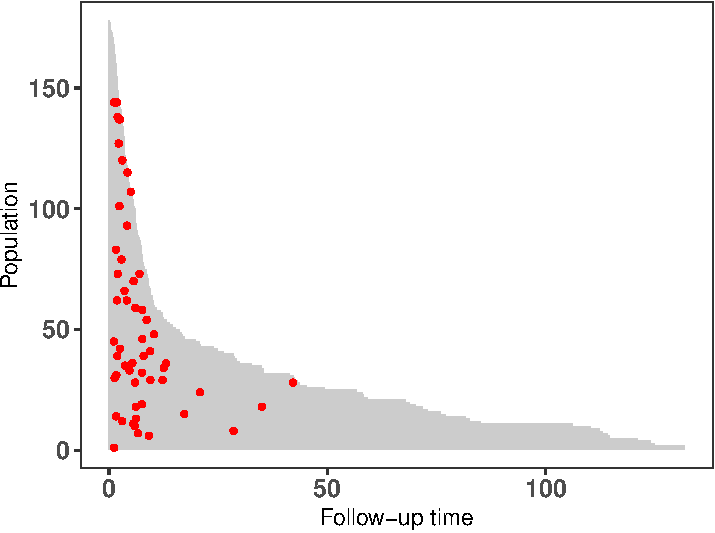
\includegraphics{casebase_jss_files/figure-latex/compPop1-1} 

}

\caption{\label{fig:compPop1}Population-time plot for the stem-cell transplant study. The points represent the event of interest (i.e., relapse).}\label{fig:compPop1}
\end{figure}
\end{CodeChunk}

\begin{CodeChunk}
\begin{figure}

{\centering 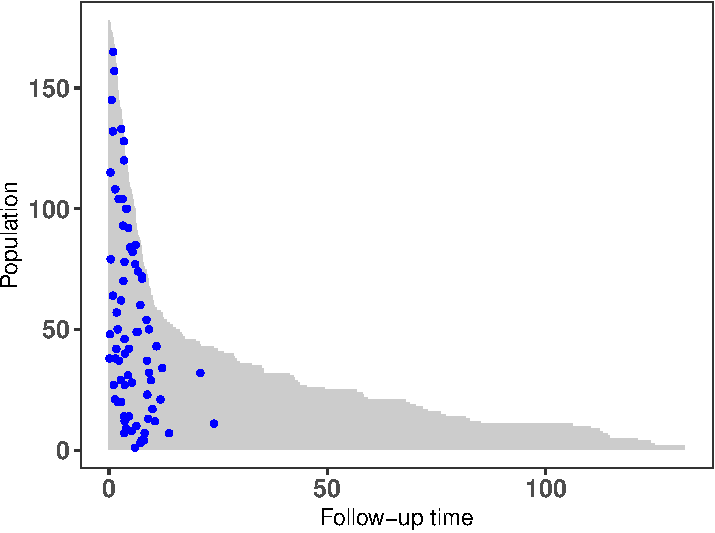
\includegraphics{casebase_jss_files/figure-latex/compPop2-1} 

}

\caption{\label{fig:compPop2}Population-time plot for the stem-cell transplant study. The points represent the competing events.}\label{fig:compPop2}
\end{figure}
\end{CodeChunk}

Our main objective is to compute the absolute risk of relapse for a
given set of covariates. First, we fit a smooth hazard to the data; for
the sake of this example, we opted for a linear term for time:

\begin{CodeChunk}

\begin{CodeInput}
R> model_cb <- fitSmoothHazard(
R+     Status ~ ftime + Sex + D + Phase + Source + Age, 
R+     data = bmtcrr, 
R+     ratio = 100, 
R+     time = "ftime")
\end{CodeInput}
\end{CodeChunk}

From the fit object, we can extract both the hazard ratios and their
corresponding confidence intervals:

\begin{CodeChunk}

\begin{tabular}{l|r|l}
\hline
Covariates & HR & 95\% CI\\
\hline
Sex & 0.71 & (0.41, 1.24)\\
\hline
Disease & 0.52 & (0.28, 0.93)\\
\hline
Phase (CR2 vs. CR1) & 1.17 & (0.47, 2.93)\\
\hline
Phase (CR3 vs. CR1) & 1.78 & (0.46, 6.91)\\
\hline
Phase (Relapse vs. CR1) & 4.45 & (2.07, 9.57)\\
\hline
Source & 1.64 & (0.54, 5)\\
\hline
Age & 0.99 & (0.97, 1.02)\\
\hline
\end{tabular}

\end{CodeChunk}

As we can see, the only significant hazard ratio is the one associated
with the phase of the disease at transplant. More precisely, being in
relapse at transplant is associated with a hazard ratio of 3.92 when
compared to CR1.

Given our estimate of the hazard function, we can compute the absolute
risk curve for a fixed covariate profile. We performed this computation
for a 35 year old woman who received a stem-cell transplant from
peripheral blood at relapse. We compared the absolute risk curve for
such a woman with acute lymphoblastic leukemia with that for a similar
woman with acute myeloblastic leukemia. Figure \ref{fig:compAbsrisk}
shows these two curves as a function of time. This figure also shows the
Kaplan-Meier estimate fitted to the two disease groups (ignoring the
other covariates).

\begin{CodeChunk}

\begin{CodeInput}
R> # Pick 100 equidistant points between 0 and 60 months
R> time_points <- seq(0, 60, length.out = 100)
R> 
R> # Data.frame containing risk profile
R> newdata <- data.frame("Sex" = factor(c("F", "F"), 
R+                                      levels = levels(bmtcrr[,"Sex"])),
R+                       "D" = c("ALL", "AML"),
R+                       "Phase" = factor(c("Relapse", "Relapse"), 
R+                                        levels = levels(bmtcrr[,"Phase"])),
R+                       "Age" = c(35, 35),
R+                       "Source" = factor(c("PB", "PB"), 
R+                                         levels = levels(bmtcrr[,"Source"])))
R> 
R> # Estimate absolute risk curve
R> risk_cb <- absoluteRisk(object = model_cb, time = time_points,
R+                         method = "montecarlo", newdata = newdata)
\end{CodeInput}
\end{CodeChunk}

\begin{CodeChunk}
\begin{figure}

{\centering \includegraphics{casebase_jss_files/figure-latex/unnamed-chunk-6-1} 

}

\caption{\label{fig:compAbsrisk}Absolute risk curve for a fixed covariate profile and the two disease groups. The estimate obtained from case-base sampling is compared to the Kaplan-Meier estimate.}\label{fig:unnamed-chunk-6}
\end{figure}
\end{CodeChunk}

\section{Case study 3: Vaccination study (recurrent
events)}\label{case-study-3-vaccination-study-recurrent-events}

\begin{itemize}
\tightlist
\item
  Give a more complex example of sampling; time-dependent exposure

  \begin{itemize}
  \tightlist
  \item
    Sampling needs to be done manually, but fitting function can still
    be used
  \end{itemize}
\end{itemize}

\section{Discussion}\label{discussion}

\bibliography{casebase_references.bib}


\end{document}

